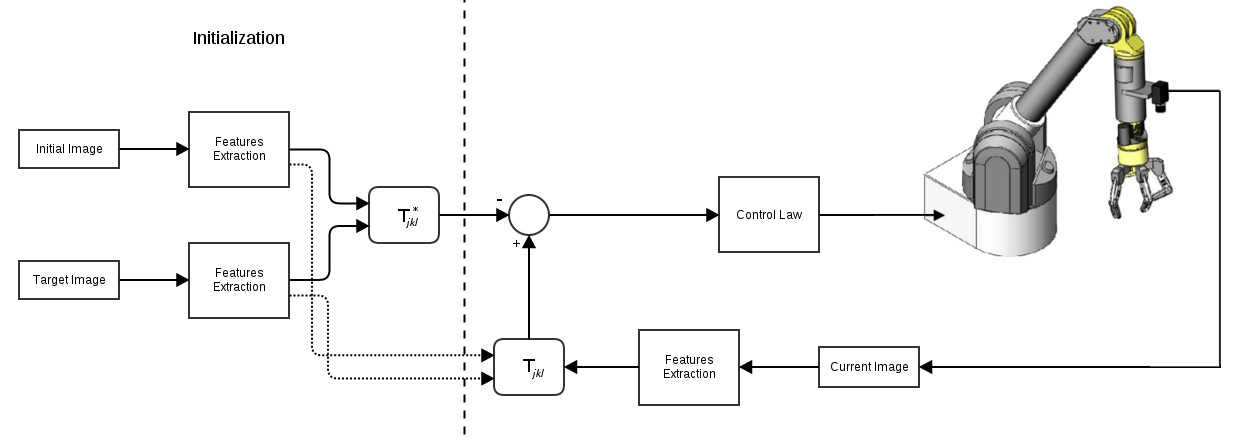
\includegraphics[width=.9\textwidth,height=40mm]{figures/vsttloop.png}
\begin{multicols}{2}
  Since the trifocal tensor is computed up to a scale factor, we propose a normalization step to get a fixed scale. The normaliztion factors $\mathcal{T}_{kN}$ are used to obtain the normalized tensor $T_{jkl}$.
\begin{gather*}
  T_{jkl} = \frac{\mathcal{T}_{jkl}}{\mathcal{T}_{kN}}, \mathcal{T}_{kN} = (\sum_n \sum_m {\mathcal{T}_{nkm}}^{2}) ^{\frac{1}{2}}
\end{gather*}
The derivation of the normalized trifocal tensor corresponding interaction matrix $L_{T_{(jkl)}}$ is then:
\begin{align*}
  \dot{T}_{(jkl)} &= L_{T_{(jkl)}} u_c\\
                  &= \frac{\textcolor{lightblue}{\tensor[^{i}]{R}{_{c^{*}(lj)}}}}{\mathcal{T}_{kN}}v_{c(k)} +\sum_{m} {[\omega_{c}]}_{\times(km)} T_{(jml)}\\&-T_{(jkl)}(\sum_n \sum_{m}T_{nkm}\frac{ \textcolor{lightblue}{\tensor[^{i}]{R}{_{c^{*}(mn)}}} }{\mathcal{T}_{kN}}) v_{c(k)} \\&+ T_{(jkl)}(\sum_n \sum_{m}T_{nkm}T_{nhm})\omega_{(g)} \\&- T_{(jkl)}(\sum_n \sum_{m}T_{nkm}T_{ngm})\omega_{(h)}\\
  \text{where } g &= k\%3 +1, h = (k+1)\%3 +1
  \end{align*}
With all elements defined, the control law is computed, and the visual servoing task is as follows:
\begin{gather*}
    e = T_{(jkl)} - T_{(jkl)}^{*}\\
  u_c = -\lambda L_{T_{(jkl)}}^{+} e
\end{gather*}
\begin{enumerate}\compresslist
  \item At initialization, the desired tensor $T_{(jkl)}^{*}$ is computed from feature correspondences across the three images.
  \item The current tensor $T_{(jkl)}$ is computed inside the visual servoing loop at each iteration.
  \item The interaction matrix $L_{T_{(jkl)}}$ is computed using the current tensor.
  \item The required velocities to drive the camera to the desired pose are computed with the new error value and the pseudo-inverse of the interaction matrix.
  \item The system converges and the loop is terminated when the camera reaches the desired pose, means the error value is less than a defined threshold.
\end{enumerate}
\end{multicols}
